\PassOptionsToPackage{usenames, dvipsnames}{xcolor}
\documentclass[tikz, 10pt]{standalone}
\usepackage{fontspec}
  \defaultfontfeatures{Ligatures={NoCommon, NoDiscretionary, NoHistoric, NoRequired, NoContextual}, Mapping=tex-text}
  \setmainfont{Times New Roman}
\usepackage{xcolor}
\usepackage{graphicx}
\usepackage{relsize}
\usepackage{tikz, tikz-qtree}
	\usetikzlibrary{shapes, arrows, backgrounds, fit, positioning}

\begin{document}
  \begin{tikzpicture}[node distance=4em, anchor=west, align=flush center, POINT/.style={black, very thick, fill=red, fill opacity=.65}, FLOW/.style={->, very thick}, LABEL/.style={draw, fill=yellow!80, inner sep=.75em}, scale = 2, transform shape]
  	\node{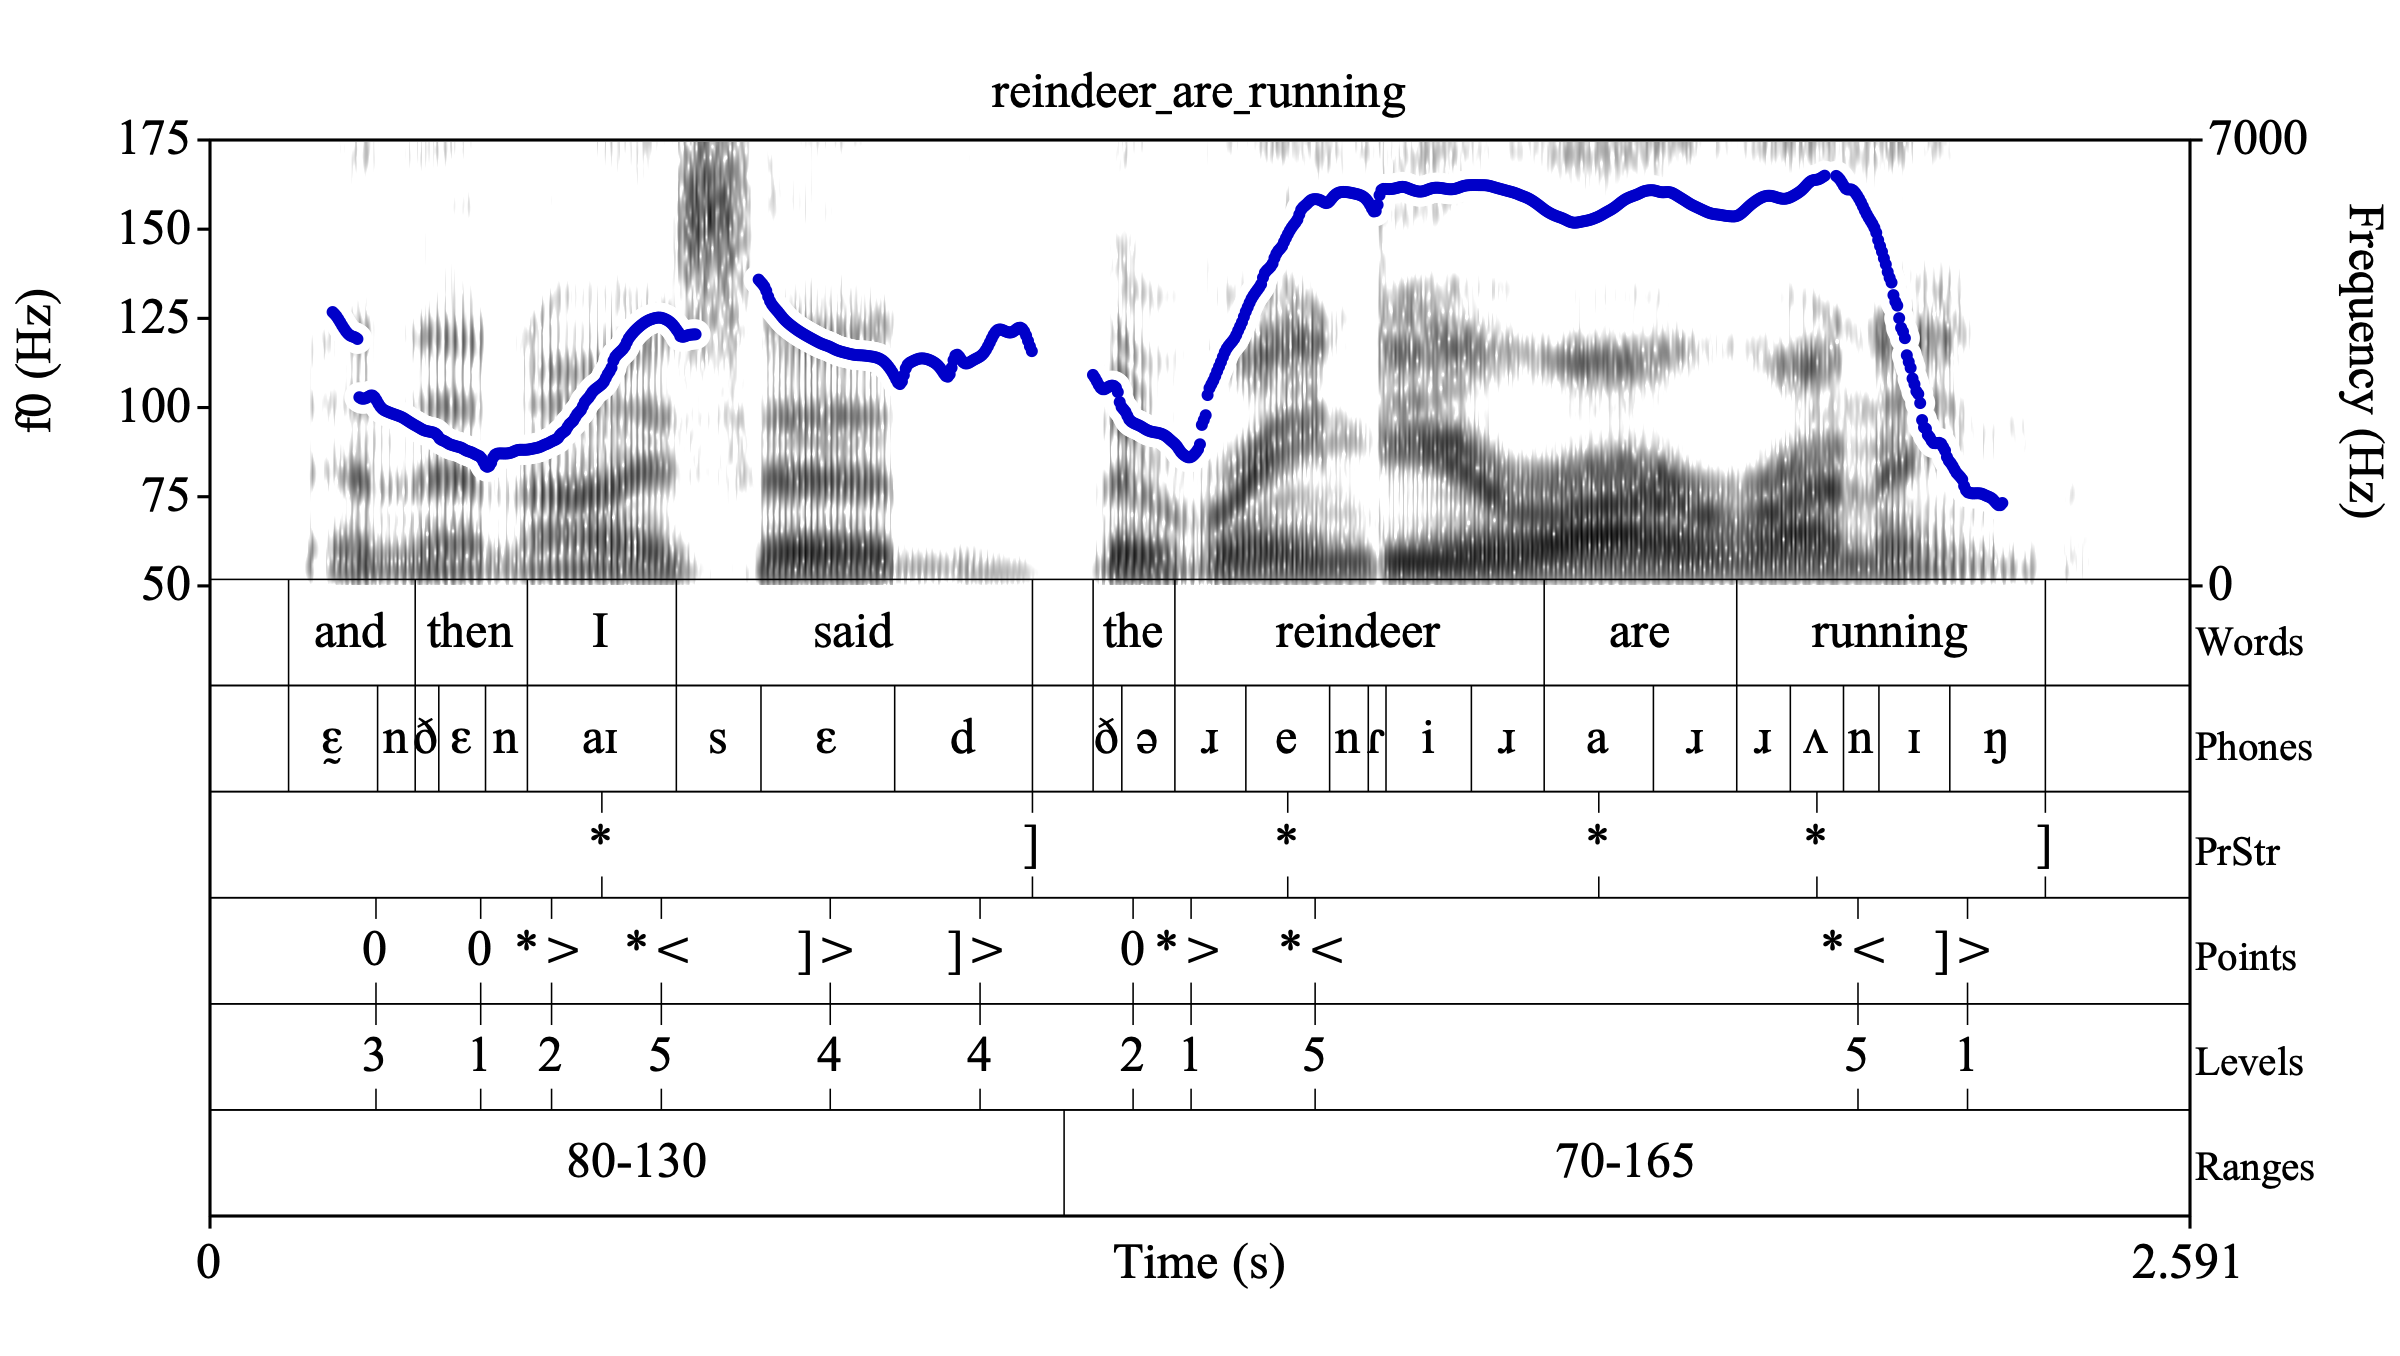
\includegraphics[width=25em]{reindeer_are_running.png}};
%    \draw [black, fill=violet!30, opacity=.5] (1, 0.7) rectangle (4.05, 0.84);
%    \draw [black, fill=blue!30, opacity=.5] (1, 0.84) rectangle (4.05, 0.98);
%    \draw [black, fill=green!30, opacity=.5] (1, 0.98) rectangle (4.05, 1.12);
%    \draw [black, fill=yellow!30, opacity=.5] (1, 1.12) rectangle (4.05, 1.26);
%    \draw [black, fill=red!30, opacity=.5] (1, 1.26) rectangle (4.05, 1.4);
%
%    \draw [black, fill=violet!30, opacity=.5] (4.05, 0.57) rectangle (8, 0.83);
%    \draw [black, fill=blue!30, opacity=.5] (4.05, 0.83) rectangle (8, 1.09);
%    \draw [black, fill=green!30, opacity=.5] (4.05, 1.09) rectangle (8, 1.35);
%    \draw [black, fill=yellow!30, opacity=.5] (4.05, 1.35) rectangle (8, 1.61);
%    \draw [black, fill=red!30, opacity=.5] (4.05, 1.61) rectangle (8, 1.87);
    \filldraw[POINT] (1.5, 1.02) circle (1.5pt);
	\draw[red, opacity=.35] (1.5, -1.2) -- (1.5, 1.96);
    \filldraw[POINT] (1.88, 0.8) circle (1.5pt);
	\draw[red, opacity=.35] (1.88, -1.2) -- (1.88, 1.96);
    \filldraw[POINT] (2.14, 0.87) circle (1.5pt);
	\draw[red, opacity=.35] (2.14, -1.2) -- (2.14, 1.96);
    \filldraw[POINT] (2.54, 1.32) circle (1.5pt);
	\draw[red, opacity=.35] (2.54, -1.2) -- (2.54, 1.96);
    \filldraw[POINT] (3.16, 1.21) circle (1.5pt);
	\draw[red, opacity=.35] (3.16, -1.2) -- (3.16, 1.96);
    \filldraw[POINT] (3.71, 1.18) circle (1.5pt);
	\draw[red, opacity=.35] (3.71, -1.2) -- (3.71, 1.96);
    \filldraw[POINT] (4.27, .94) circle (1.5pt);
	\draw[red, opacity=.35] (4.27, -1.2) -- (4.27, 1.96);
    \filldraw[POINT] (4.48, .81) circle (1.5pt);
	\draw[red, opacity=.35] (4.48, -1.2) -- (4.48, 1.96);
    \filldraw[POINT] (4.94, 1.75) circle (1.5pt);
	\draw[red, opacity=.35] (4.94, -1.2) -- (4.94, 1.96);
    \filldraw[POINT] (6.92, 1.77) circle (1.5pt);
	\draw[red, opacity=.35] (6.92, -1.2) -- (6.92, 1.96);
    \filldraw[POINT] (7.33, .69) circle (1.5pt);
	\draw[red, opacity=.35] (7.33, -1.2) -- (7.33, 1.96);
  \end{tikzpicture}
\end{document}